\documentclass{prettytex/ox/mmsc-special-topic}

\setlength{\headheight}{19.53pt}
\setlength{\headsep}{1.8em}
\setlength{\belowcaptionskip}{-12pt}
\setminted{fontsize=\footnotesize}
\AfterEndEnvironment{minted}{\vspace*{-0.8cm}}
\renewcommand{\operatorcolor}{black}

\addbibresource{sources.bib}
\tikzexternalize[prefix=tikz/]

\newcommand{\topictitle}{Battery Computing}
\newcommand{\candidatenumber}{1072462}
\newcommand{\course}{Scientific Computing}

\title{\topictitle}
\author{Candidate \candidatenumber}
\date{\today}

\makenoidxglossaries
\newacronym{pde}{PDE}{Partial Differential Equation}
\newacronym{ode}{ODE}{Ordinary Differential Equation}

% TODO: verify oxidation reaction

\begin{document}
  \pagestyle{plain}
  \mmscSpecialHeader[casestudy]

  \begin{abstract}
    \label{abstract}
    This work shall attempt to
    \vspace*{0.2cm}

    \noindent
    \textbf{Our Goal:}
    Numerically obtain the solution $\{a(x, T), b(x, T)\}$ of
    \vspace*{-0.2cm}
    $$\begin{cases}
        % \setstretch{1}
        \frac{\partial a}{\partial t} = D_a \frac{\partial^2 a}{\partial x^2}, & a: \R^+ \times [0, T] \mapsto [0, 1],\, T \in \R^+,\; D_a \in \R^+, \\[-0.2em]
        \frac{\partial b}{\partial t} = D_b \frac{\partial^2 b}{\partial x^2}, & b: \R^+ \times [0, T] \mapsto [0, 1],\, D_b \in \R^+,               \\[-0.2em]
        a(\infty, t) = 1,\; b(\infty, t) = 0                                   & \forall t \in [0, T]                                                \\[-0.2em]
        a(x, 0) = 1,\;\; b(x, 0) = 0                                           & \forall x \in (0, \infty)                                           \\[-0.2em]
        a(0, t) = 0,\; \frac{\partial a}{\partial x} + D \frac{\partial b}{\partial x} = 0
      \end{cases}$$
    \vspace*{0.05cm}

    The implementation bla bla
  \end{abstract}

  \begin{figure}[H]
    \centering
    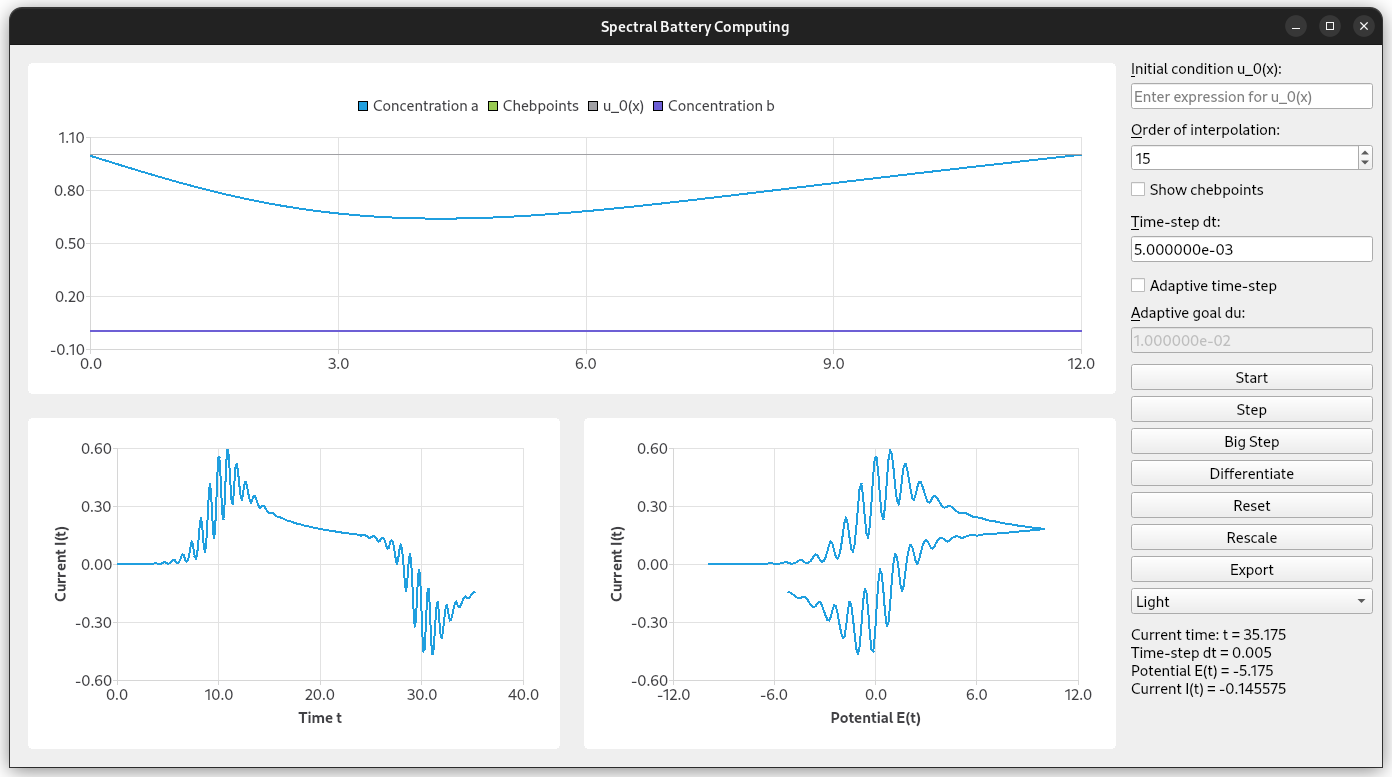
\includegraphics[width=\linewidth]{figures/screenshot.png}
    \caption{Graphical User Interface}
  \end{figure}

  \pagebreak
  \pagestyle{normal}

  \tableofcontents
  \pagebreak

  \section{Problem Introduction}
  Energy storage and its associated challenges are clearly among the most relevant questions, not only for the industrial but also the private sector.
  Politically, many nations in the world are steering towards greener energy supplies.
  Renewable energy sources such as wind and sun usually have a fundamental issue however, their availability is subject to an immense amount of fluctuation, which the energy grid must compensate through short- and long-term energy storage.

  Long-term solutions include for example pumped-storage hydroelectricity facilities, but these must be complemented with short-term storage approaches such as Lithium-Ion or Lithium-Iron-Phosphate ($\text{LiFePO}_4$) batteries.
  Most modern batteries exploit electrochemical reactions to relate electrical potentials with chemical potentials and their associated difference ($\rightarrow$ voltage).
  The oxidation reaction we considere here is
  $$A \Rightarrow B + e^-?$$
  where $A$ and $B$ can be any chemicals and $e^-$ is an electron \parencite{Gavaghan2000Jan}.

  More bla bla later on.

  \begin{figure}[H]
    \centering
    \inputtikz{figure1}
    \caption{Wohoo.}
    \label{fig:fig1}
  \end{figure}

  \begin{figure}[H]
    \centering
    \inputtikz{figure2}
    \caption{Schematic of the finite different scheme where ... are the nodes specified by initial conditions, and ... are the nodes specified by boundary conditions.}
    \label{fig:fig2}
  \end{figure}

  As stated on \Cpageref{abstract}, we consider the following \gls{pde}s in the concentrations $a, b \in \C^2(\Omega)$
  \begin{align}
    \label{eq:pde-a} \frac{\partial a}{\partial t} = D_a \frac{\partial^2 a}{\partial x^2} \\
    \label{eq:pde-b} \frac{\partial b}{\partial t} = D_b \frac{\partial^2 b}{\partial x^2}
  \end{align}

  \subsection{Chronoamperometry}
  \subsection{DC Voltammetry}
  \subsection{AC Voltammetry}

  \section{Mathematical Background}
  Let $\N$ denote the nonnegative integers, so $0 \in \N$.
  Similarly, let $\R^+ = [0, \infty)$ denote the nonnegative real numbers.
  \autoref{fig:fig1}.

  \subsection{Laplace Integral Transform}
  What is Laplace?

  Laplace transforms are especially valuable for physical systems as many of them expose exponentially decaying and/or periodic behaviours which the Laplace transform is well-suited for due to the form of its kernel.
  Decaying behaviour is captured by the real component of the argument $s$, $\Re(s)$, whereas periodicities are captured by the imaginary part $\Im(s)$\footnote{Consider for comparision the Fourier transform $\cF(a)(\omega) := \int_{-\infty}^{\infty} a(t) \e^{\i \omega t} \,\ddt$ which captures periodic frequencies, where the kernel automatically follows multiplication along the unit circle due to the imaginary-valued exponent $\i\omega t$ (the argument $\omega \in \R$ is real-valued). Intuitively, the Laplace transform coincides with the Fourier transform if evaluated at $s = \i \omega$.}.

  \begin{theorem}{Laplace Transform of the Derivative}{laplace-diff}
    Given a function $a(t)$ and a corresponding Laplace-transform $\hat{a}(s) = \cL\{a\}(s)$, the transform of the derivative $a'(t)$ of the original function is given by
    $$\cL\{a'\}(s) = \cL\left\{t \mapsto \frac{\partial a}{\partial t}\right\}(s) = s\hat{a}(s) - a_0\,,$$
    where $a_0 := a(t=0)$.
  \end{theorem}

  \begin{proof}
    Proof for Laplace's differentiation theorem.
  \end{proof}


  \subsection{Chebyshev Polynomials}
  Proof of $U_k(-1)$'s value.

  \section{Finite Differences}
  Construct $A \vec{x} = \vec{b}$.

  \subsection{Results}

  \section{Analytical Approaches}
  \subsection{Similarity Solution}
  \subsection{Integral Equation}
  \subsubsection{Derivation using the Laplace Transform}
  As mentioned above, the Laplace Integral Transform is especially useful in the context of differential equations, mostly due to \Cref{thm:laplace-diff}.
  Applying it to our \textit{partial} differential diffusion equation \Cref{eq:pde-a} transforms the problem into one of solving an \textit{ordinary} differential equation.
  Similarly, \glstext{ode}s could be turned into algebraic equations using a similar approach.

  Starting from \Cref{eq:pde-a}

  \subsubsection{Numerical Solution}

  \section{Spectral Method}
  From the definition of Chebyshev polynomials $T_k(x) = \cos(k\theta)$, we can derive that
  $$\frac{\dd T_k}{\ddx} = \frac{\dd T_k}{\dd\theta} \frac{\dd\theta}{\ddx} = ... = k U_{k-1}(x)\,,$$
  where $U_k: [-1, 1] \mapsto \R$ denote the Chebyshev polynomials of the second kind, which in turn are defined by
  $$U_k(\cos \theta) \sin(\theta) = \sin\left((n+1) \theta\right)\,.$$

  In order to enforce a von-Neumann boundary condition on the left and a Dirichlet boundary condition on the right,
  we are interested in explicitly setting coefficients $a_k$ such that
  $$a_x(-1, t) = \frac{\dd a}{\ddx}\Big|_{x=-1} = \tilde{l} \quad \text{ and } \quad a(1) = r, \quad \text{ where } \quad \tilde{l}, r \in \R\,.$$

  Using the Chebyshev series ansatz
  $$a(x, t) = \sum_{k=0}^{N-1} a_k^{(t)} T_k(x)$$
  we have that
  $$\frac{\dd a}{\ddx} = \sum_{k=0}^{N-1} a_k^{(t)} \frac{\dd T_k}{\ddx}(x)\,,$$
  so we are interested in
  $$a_x(-1, t) = \frac{\dd a}{\ddx}\Big|_{x=-1} = \sum_{k=0}^{N-1} a_k^{(t)} \frac{\dd T_k}{\ddx}\Big|_{x=-1} = \sum_{k=0}^{N-1} a_k^{(t)} k U_{k-1}(-1)\,.$$

  Following from TODO (explained on Wikipedia), we know that
  $$U_k(-1) = (-1)^k (k+1) \quad \text{ and } \quad T_k(1) = 1 \quad \forall k \in \N\,,$$
  which turns our conditions into algebraic conditions w.r.t. the coefficients $a_k^{(t)}$,
  $$a_x(-1, t) = \frac{\dd a}{\ddx}\Big|_{x=-1} = \sum_{k=0}^{N-1} a_k^{(t)} k^2 (-1)^{k-1} \overset{!}{=} \tilde{l} \quad \text{ and } \quad a|_{x=1} = \sum_{k=0}^{N-1} a_k^{(t)} \overset{!}{=} r\,.$$

  Knowing that the heat equation Forward Euler numerical scheme modifies all but the two highest-degree coefficients in the series, we expand:
  \begin{align*}
    a_x(-1, t) = \sum_{k=0}^{N-1} a_k^{(t)} T_k'(-1) =   & \overbrace{-\sum_{k=0}^{N-3} a_k^{(t)} k^2 (-1)^{k}}^{:= \Sigma_3} - (N-2)^2 (-1)^{N-2} a_{N-2}                  \\
                                                         & -(N-1)^2 (-1)^{N-1} a_{N-1} = l\,,                                                                               \\
    a(1, t)    = \sum_{k=0}^{N-1} a_k^{(t)} T_k(1)     = & \underbrace{\sum_{k=0}^{N-3} a_k^{(t)}}_{:= \Sigma_2}              + a_{N-2}                    + a_{N-1} = r\,,
  \end{align*}

  \subsection{Enforcing Boundary Conditions}
  Von Neumann on the left

  \subsection{Implicit Euler}

  \subsection{Implementation}
  The solver was implemented in C++.

  % \inputminted{cpp}{../SpectralSolver/Solver.h}

  \subsection{Results}
  Chronoamperometry,
  DC Voltammetry,
  AC Voltammetry

  \section{Conclusion}

  \pagebreak
  \printbibliography
  \printnoidxglossary[type=acronym]
\end{document}
